\section{Tokamaks}
\begin{frame}{Tokamaks}
    The Tokamak uses coils to control the plasma in the torus-shape chamber.
    \begin{figure}
        \begin{subfigure}{0.5\textwidth}
            \centering
            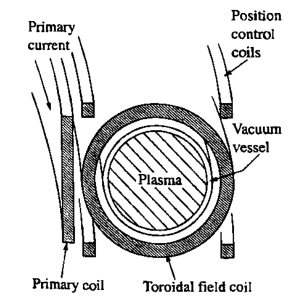
\includegraphics[width=\textwidth]{figures/tokamak-coils.png}
            \caption{Arrangement of coils in a tokamak.}
        \end{subfigure}%
        \begin{subfigure}{0.5\textwidth}
            \centering
            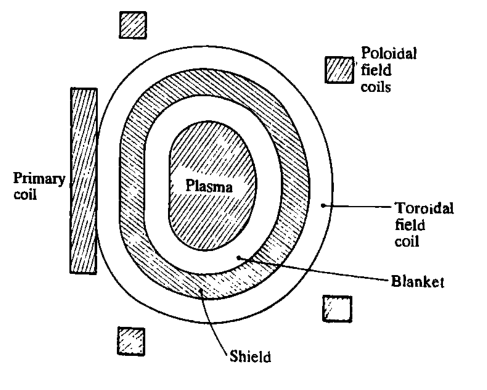
\includegraphics[width=\textwidth]{figures/tokamak-coils-layout.png}
            \caption{Blanket (compound containing Li) is used to absorb the thermonuclear energy and also for tritium breeding.}
        \end{subfigure}
    \end{figure}
\end{frame}

\begin{frame}{Magnetic Field}
    The poloidal and toroidal magnetic field are essential to stabilize the plasma
    \begin{figure}
        \centering
        \begin{subfigure}{0.45\textwidth}
            \centering
            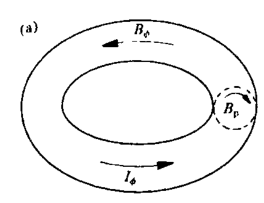
\includegraphics[width=\textwidth]{figures/tokamak-magnetic-field-a.png}
            \caption{Toroidal magnetic field $B_\phi$, and poloidal magnetic field $B_p$ due to toroidal current $I_\phi$.}
        \end{subfigure}%
        \begin{subfigure}{0.45\textwidth}
            \centering
            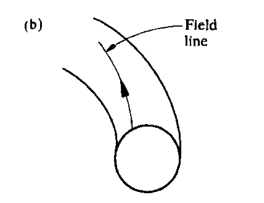
\includegraphics[width=\textwidth]{figures/tokamak-magnetic-field-b.png}
            \caption{Combination of $B_\phi$ and $B_p$ causes field lines to twist around plasma.}
        \end{subfigure}
    \end{figure}
\end{frame}

\begin{frame}{Tokamak Reactor - Structure}
    In the classical design of tokamak reactor, we only replace the energy source by a tokamak, for the rest of the structure we have mature industrial solutions already.
    \begin{figure}
        \centering
        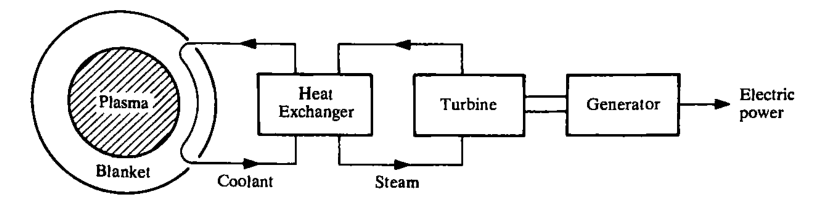
\includegraphics[width=\textwidth]{figures/tokamak-reactor.png}
        \caption{Thermonuclear power absorbed in blanket would be converted into electric power by conventional means.}
    \end{figure}
\end{frame}

\begin{frame}{Tokamak Reactor - Power}
    The power density of the D-T reaction is given by Eq.(\ref{eq:thermonuclear-power-density}), so
    \begin{equation}
        P = \frac{\pi}{2}\varepsilon \int n^2\expval{\sigma v}R dS
    \end{equation}
    where $S$ is an area element of the poloidal cross-section. We can simplify it by taking $R$ as constant and $\bar{a}=(ab)^{1/2}$. Moreover, $\expval{\sigma v}$ can be approximated by $1.1\times 10^{-24} T^2$, and the pressure profile can be taken as $nT = \hat{n}\hat{T}(1-r^2/\bar{a}^2)^\nu$, so the total power
    \begin{equation}
        P = \frac{0.15}{2\nu+1}Rab\left(\frac{\hat{n}}{10^20}\right)^2\hat{T}^2
    \end{equation}
    where the unit of $\hat{T}$ is keV.
\end{frame}

\begin{frame}{Tokamak Reactor - Impurities}
    There are two types of impurities:
    \begin{itemize}
        \item Ions coming from solid surfaces (walls). Need to avoid this since it causes plasma energy loss through radiation.
        \item $\alpha$-particles, $^4$He. The $\alpha$-particles are the byproduct of fusion reaction. It is believed that a magnetic divertor is required to guide the "helium ash" to a "target" surface well separated from the plasma, and to restrict the impurity back-flow.
    \end{itemize}
\end{frame}
